\documentclass{beamer}

\usepackage[utf8]{inputenc} %Eingabecode/Schriftsatz
\usepackage[ngerman]{babel} %Schriftsatz - neue deutsche Rechtschreibung
\usepackage[T1]{fontenc} %Ausgabecode/Schriftsatz
\usepackage{lmodern}

%%%%%%%%%%%%%%%%%%%%%%%%%%%%%%%%%%%%%%%%%%%%%%%%%%%%%%%%%%
\usetheme{Warsaw}

\makeatletter
\newcommand\titlegraphicii[1]{\def\inserttitlegraphicii{#1}}
\titlegraphicii{}
\setbeamertemplate{title page}
{
  \vbox{}
   {\usebeamercolor[fg]{titlegraphic}\inserttitlegraphic\hfill\inserttitlegraphicii\par}
  \begin{centering}
    \begin{beamercolorbox}[sep=8pt,center]{institute}
      \usebeamerfont{institute}\insertinstitute
    \end{beamercolorbox}
    \begin{beamercolorbox}[sep=8pt,center]{title}
      \usebeamerfont{title}\inserttitle\par%
      \ifx\insertsubtitle\@empty%
      \else%
        \vskip0.25em%
        {\usebeamerfont{subtitle}\usebeamercolor[fg]{subtitle}\insertsubtitle\par}%
      \fi%     
    \end{beamercolorbox}%
    \vskip1em\par
    \begin{beamercolorbox}[sep=8pt,center]{date}
      \usebeamerfont{date}\insertdate
    \end{beamercolorbox}%\vskip0.5em
    \begin{beamercolorbox}[sep=8pt,center]{author}
      \usebeamerfont{author}\insertauthor
    \end{beamercolorbox}
  \end{centering}
  %\vfill
}
\makeatother
\author{\itshape Projekt von: \\ Björn Sölter und Jonas Hill}
\title{Unity Game Studio}
\subtitle{Get them of the f****** Grid}
%\institute{Department \\ University}
\date{\today}
\centering
\titlegraphic{
\includegraphics[width=0.33\textwidth, angle=0]{Abbildungen/UniMR.png}}

\begin{document}

\begin{frame}[plain]
\maketitle
\small
{\centering\itshape Dozenten:\par}
Sebastian Lieb \& Thorsten Thormählen
\end{frame}

\clearpage

\section{I}
\begin{frame} %%Eine Folie
  \frametitle{Ziel des Spiels} %%Folientitel
	
	\begin{minipage}[]{0.45\textwidth}
		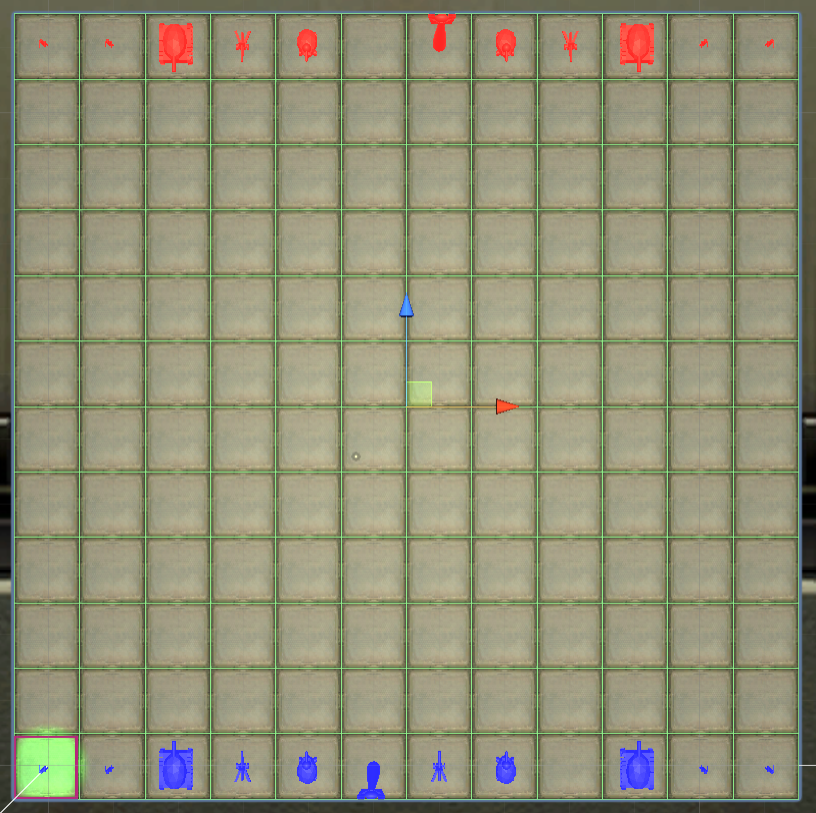
\includegraphics[width=\textwidth]{Abbildungen/GameTop.PNG}
	\end{minipage}
	\begin{minipage}[]{0.45\textwidth}
		\begin{itemize}
			\item durch strategisches Positionieren von und Angreifen mit verschiedenen Einheiten
			\item eigenen König schützen und den gegnerischen König stürzen
		\end{itemize}
	\end{minipage}
	
\end{frame}

\begin{frame} %%Eine Folie
  \frametitle{Ziel des Spiels} %%Folientitel
	
	\begin{minipage}[]{0.45\textwidth}
		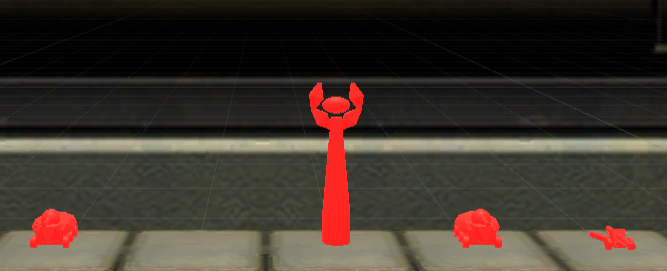
\includegraphics[width=\textwidth]{Abbildungen/King.PNG}
	\end{minipage}
	\begin{minipage}[]{0.45\textwidth}
		\begin{itemize}
			\item König des roten Spielers
		\end{itemize}
	\end{minipage}
	
	\begin{minipage}[]{0.45\textwidth}
		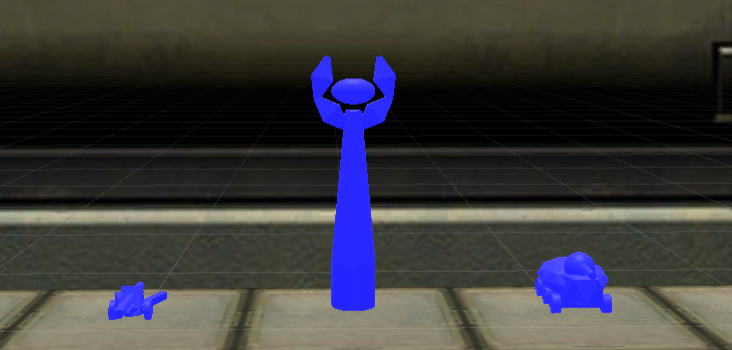
\includegraphics[width=\textwidth]{Abbildungen/King2.PNG}
	\end{minipage}
	\begin{minipage}[]{0.45\textwidth}
		\begin{itemize}
			\item König des blauen Spielers
		\end{itemize}
	\end{minipage}
	
\end{frame}

\section{II}
\begin{frame} %%Eine Folie
  \frametitle{Wie wird gespielt?} %%Folientitel
	
	\begin{itemize}
		\item Bewegen einer beliebigen eigenen Figur im Rahmen ihrer Bewegungs-Reichweite
		\item Angreifen einer beliebigen gegnerischen Figur im Rahmen ihrer Angriffs-Reichweite
		\item Abgeben des Zuges an den Gegner
	\end{itemize}
	
\end{frame}

\begin{frame} %%Eine Folie
  \frametitle{Wie wird gespielt?} %%Folientitel
	
	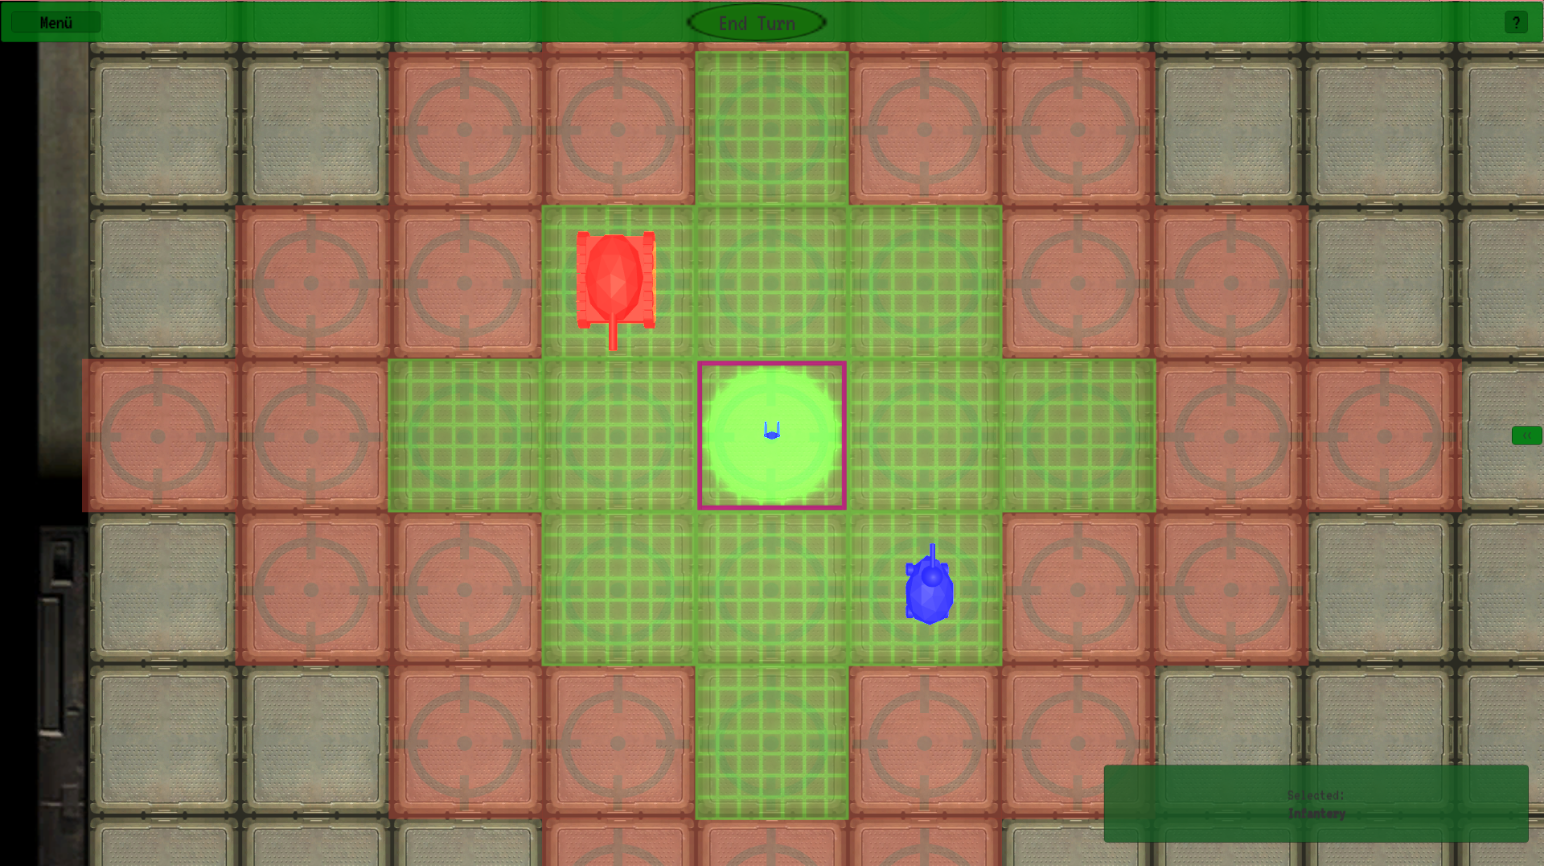
\includegraphics[width=\textwidth]{Abbildungen/Ranges.PNG}
	
\end{frame}

\section{III}
\begin{frame} %%Eine Folie
  \frametitle{Objekte} %%Folientitel
		Verschieden Einheiten mit verschiedenen Fähigkeiten
		
		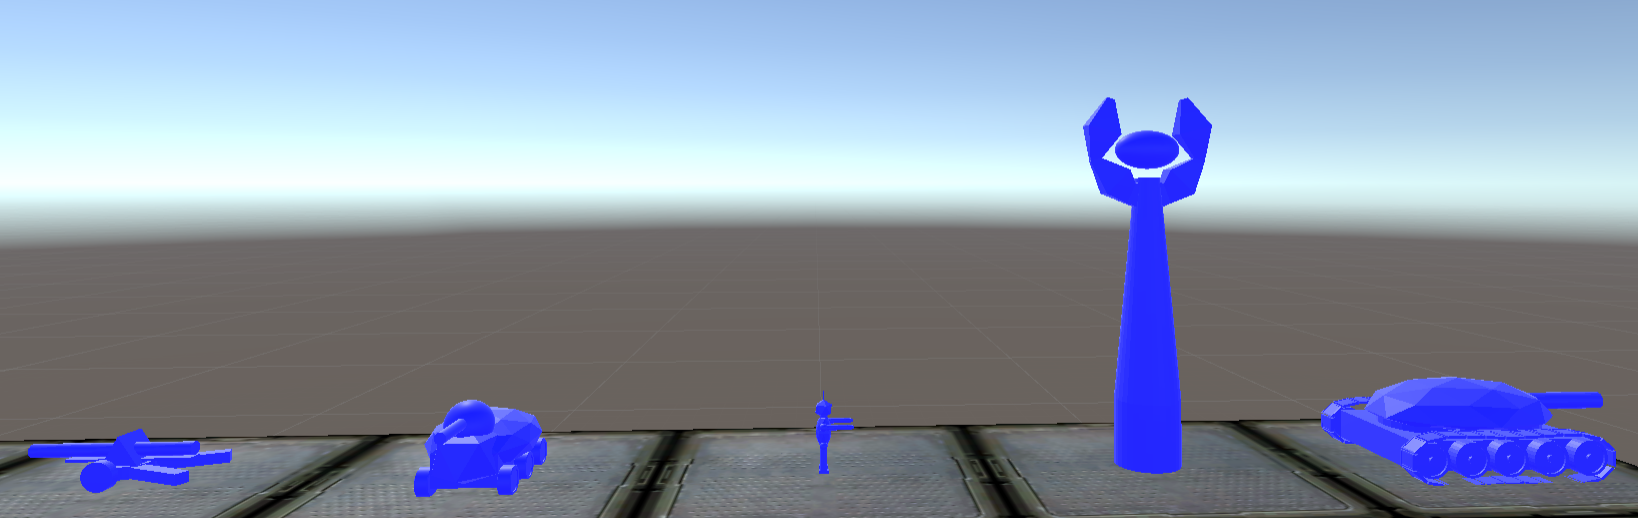
\includegraphics[width=0.9\textwidth]{Abbildungen/Objects.PNG}
\end{frame}

\section{IV}
\begin{frame} %%Eine Folie
  \frametitle{Features} %%Folientitel
  
	\begin{minipage}[]{0.45\textwidth}
		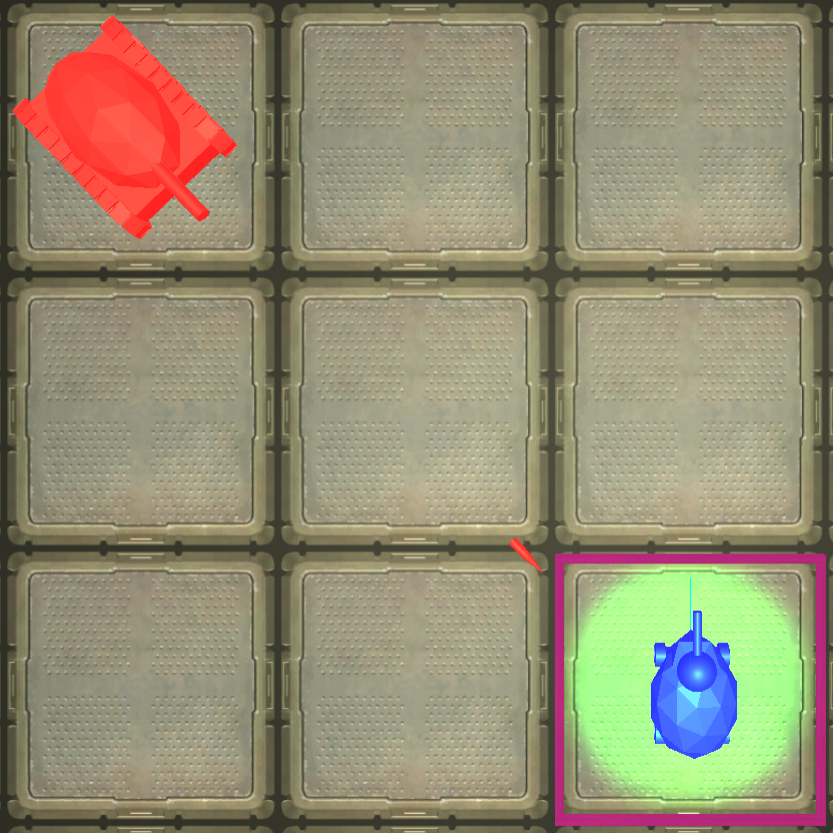
\includegraphics[width=\textwidth]{Abbildungen/BulletAndAngle.PNG}
	\end{minipage}
	\begin{minipage}[]{0.45\textwidth}
		\begin{itemize}
			\item Projektil-Generierung und Verfolgung
			\item Drehung der Objekte in Schussrichtung
			\item Schadensberechnung durch Projektil-Kollision
		\end{itemize}
	\end{minipage}
	
\end{frame}

\begin{frame} %%Eine Folie
  \frametitle{Features} %%Folientitel
  
	\begin{minipage}[]{0.45\textwidth}
		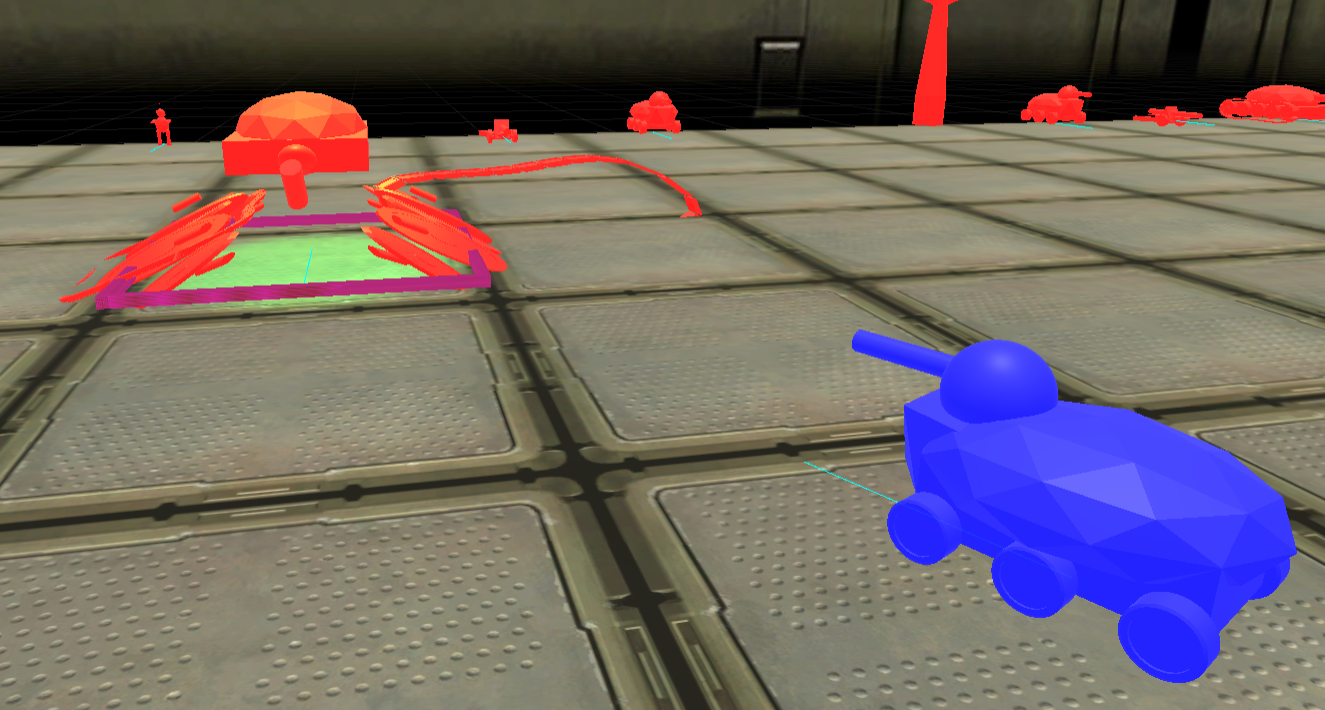
\includegraphics[width=\textwidth]{Abbildungen/Destruction.PNG}
	\end{minipage}
	\begin{minipage}[]{0.45\textwidth}
		\begin{itemize}
			\item Bei Projektil Kollision und kritischer HP
			\item Objekt Zerstörung und Löschung
		\end{itemize}
	\end{minipage}
	
\end{frame}

\section{V}
\begin{frame} %%Eine Folie
  \frametitle{Schwierigkeiten und Probleme} %%Folientitel
  
	\begin{itemize}
			\item Objekt Rotation
			
				\begin{itemize}
					\item Unterschiedliche KS von Unity und Blender
					\item keine feste Norm
				\end{itemize}
			
			\item Projektil Verfolgung
			
			\item Nutzung der Engine soviel wie nötig so wenig wie möglich
			
				\begin{itemize}
					\item Teils zu ofte Verwendung vom Unity Collision/Trigger System
					
						\begin{itemize}
							\item Arrayverwaltungen teilweise angemessener
						\end{itemize}
				
					\item Engine primär für Darstellung und Physik
					\item Scripte unabhängig von engine in C\# für Spielelogik 
				\end{itemize}
		\end{itemize}
	
\end{frame}

\begin{frame} %%Eine Folie
  \frametitle{Schwierigkeiten und Probleme} %%Folientitel
  
	\begin{itemize}
			\item Klassenstruktur
			
				\begin{itemize}
					\item Ohne Konzept etwas chaotisch
					\item manche Scripte zu überladen
				\end{itemize}
				
			\item Git
				\begin{itemize}
					\item Fluch und Segen		
				\end{itemize}
				
			\item schöene Texturierung
		\end{itemize}
	
\end{frame}


\section{VI}
\begin{frame} %%Eine Folie
  \frametitle{Ausblick} %%Folientitel
  \begin{itemize}
			\item Mehr Mechaniken
			\item Mehr Objekte, Modelle, Fähigkeiten, Effekte
			\item die Klassiker....
		\end{itemize}
\end{frame}


\begin{frame} %%Eine Folie
  \frametitle{} %%Folientitel
  \LARGE Hat Spass gemacht!
\end{frame}

\end{document}